% ============================================================================
% IEEE CONFERENCE PAPER — IEEEtran class
% Title: A Unified Machine Learning Framework for Fault Detection,
%        Classification, and Self-Healing in Three-Phase Grid-Tied Inverters
% Author: Md. Atair Rahman Alvi, BRAC University
% ============================================================================

\documentclass[conference]{IEEEtran}

% ── PACKAGES ─────────────────────────────────────────────────────────────────
\usepackage[T1]{fontenc}
\usepackage[utf8]{inputenc}
\usepackage{cite}
\usepackage{amsmath,amssymb,amsfonts}
\usepackage{algorithmic}
\usepackage{graphicx}
\usepackage{textcomp}
\usepackage{xcolor}
\usepackage{booktabs}
\usepackage{multirow}
\usepackage{array}
\usepackage{url}
\usepackage{balance}
\usepackage[hidelinks]{hyperref}

% ── COLUMN TYPE FOR TABLES ───────────────────────────────────────────────────
\newcolumntype{C}[1]{>{\centering\arraybackslash}p{#1}}
\newcolumntype{L}[1]{>{\raggedright\arraybackslash}p{#1}}
\newcolumntype{R}[1]{>{\raggedleft\arraybackslash}p{#1}}

% ── FIGURE PATH ──────────────────────────────────────────────────────────────
\graphicspath{{figures/}}

% ─────────────────────────────────────────────────────────────────────────────
\begin{document}

% ── TITLE ────────────────────────────────────────────────────────────────────
\title{A Unified Machine Learning Framework for Fault Detection,
Classification, and Self-Healing in Three-Phase Grid-Tied Inverters}

\author{
  \IEEEauthorblockN{Md. Atair Rahman Alvi}
  \IEEEauthorblockA{
    \textit{Department of Electrical and Electronics Engineering}\\
    \textit{BRAC University}\\
    Dhaka, Bangladesh\\
    alvi@bracu.ac.bd
  }
}

\maketitle

% ── ABSTRACT ─────────────────────────────────────────────────────────────────
\begin{abstract}
This paper presents a unified machine learning (ML) framework for simultaneous
fault detection, classification, and self-healing in three-phase grid-tied
inverters. Grid-tied inverters are susceptible to six critical fault conditions:
open-circuit switch fault, DC injection, grid voltage sag/swell, islanding,
phase-locked loop (PLL) desynchronization, and healthy operation. Existing
literature addresses fault classification or parameter correction in
isolation --- no prior work combines both capabilities in a unified framework
for three-phase systems. The proposed framework extracts a rich
140-dimensional feature vector from three-phase electrical measurements over
10\,ms sliding windows, encompassing mean, standard deviation, maximum,
minimum, range, RMS, and skewness of 20 electrical signals. Five
state-of-the-art baseline models are systematically benchmarked: Random
Forest (99.44\%), XGBoost (98.89\%), Shallow MLP (99.72\%), Deep MLP
(55.00\%), and Gradient Boosting (99.44\%). The proposed Residual MLP
(ResMLP)~--- incorporating four residual blocks with GELU activations and
skip connections~--- achieves 86.39\% test accuracy on CPU hardware with
validation accuracy of 98.06\% at epoch~15 on GPU, and perfect recall (1.00)
on the two most safety-critical fault classes: open-circuit switch fault and
islanding. A class-specific self-healing correction stage is integrated
downstream of the classifier, extending the healing factor concept of prior
MPC-based approaches to six fault types on a three-phase system.
\end{abstract}

\begin{IEEEkeywords}
grid-tied inverter, fault detection, fault classification, residual neural
network, machine learning, self-healing control, power quality, three-phase
inverter, model predictive control.
\end{IEEEkeywords}

% ─────────────────────────────────────────────────────────────────────────────
\section{Introduction}
% ─────────────────────────────────────────────────────────────────────────────

The accelerating integration of renewable energy sources into the utility grid
has substantially increased the deployment of grid-tied inverters. These power
electronic interfaces are critical for ensuring efficient and reliable power
transfer between distributed energy resources (DERs) and the grid. However,
grid-tied inverters are inherently susceptible to a range of electrical
faults --- open-circuit switch failures, DC current injection, grid voltage
disturbances, islanding conditions, and synchronization failures --- that
degrade power quality, violate grid codes, and may lead to costly system
failures~\cite{vazquez2014, amiri2024}.

Classical model-based fault detection relies on threshold comparisons and
residual monitoring, which are sensitive to parameter variations and operating
condition changes~\cite{sun2023}. Recent advances in AI and machine learning
have demonstrated significantly improved fault classification accuracy, with
CNNs, random forests, and hybrid architectures achieving 96--98\%
accuracy~\cite{yan2023, bhadra2025}. Nevertheless, two critical gaps persist.
First, most published ML frameworks address single-phase or DC-side faults in
PV systems, with limited work on three-phase grid-interactive
inverters~\cite{you2023}. Second, existing approaches treat fault detection and
parameter correction as separate problems.

Baker~et~al.~\cite{baker2021} proposed a self-learning MPC scheme using a
feedforward neural network to heal filter inductance mismatch in a
single-phase grid-tied inverter, reducing THD from 4.09\% to 2.58\%. While
pioneering, this work was limited to single-parameter mismatch correction and
provided no multi-class fault classification --- the classification network
achieved only 72.63\% accuracy, leading the authors to recommend the
single-network (model adaptation only) approach. Separately,
Prabakaran~et~al.~\cite{prabakaran2026} proposed the Edge-Optimized Hybrid
Attention Network (EO-HAN) achieving 97.8\% classification accuracy with
19.6\,ms inference on Jetson Nano, but providing no self-healing or
correction capability.

This paper bridges these two streams by proposing a unified ML framework
combining fault classification with class-specific self-healing correction,
applied to a three-phase grid-tied inverter with six fault categories. The
key contributions are:

\begin{enumerate}
  \item A rich 140-dimensional feature vector from three-phase measurements,
        combining 7 statistical descriptors across 20 electrical signals per
        10\,ms window --- directly extending the 8-element INP vector
        of~\cite{baker2021} to the three-phase domain.

  \item A systematic benchmark of five ML baseline models on a balanced
        120,000-sample six-class dataset, the most comprehensive comparison
        reported for three-phase inverter fault classification.

  \item A proposed Residual MLP (ResMLP) with skip connections and GELU
        activations, achieving perfect recall (1.00) on the two most
        safety-critical fault classes and demonstrating stable convergence
        where vanilla deep networks fail (55\% vs.\ 86--99\%).

  \item A unified self-healing framework extending the healing factor concept
        of~\cite{baker2021} to six fault types, providing class-specific
        correction actions integrated downstream of the classifier.
\end{enumerate}

% ─────────────────────────────────────────────────────────────────────────────
\section{Three-Phase Grid-Tied Inverter Model and Fault Scenarios}
% ─────────────────────────────────────────────────────────────────────────────

\subsection{System Model}

The three-phase grid-tied inverter interfaces a DC source with the utility
grid through a three-phase L-filter. Grid synchronization is achieved via a
PLL with a second-order generalized integrator (SOGI)-based orthogonal signal
generator. The dynamic model of the filter for phase
$j \in \{a, b, c\}$ is:

\begin{equation}
  \frac{di_j}{dt} = \frac{1}{L}\bigl[v_{\mathrm{inv},j}
    - R_{\mathrm{ESR}}\,i_j - e_{o,j}\bigr]
  \label{eq:filter}
\end{equation}

\noindent where $v_{\mathrm{inv},j}$ is the inverter bridge voltage,
$e_{o,j}$ is the grid voltage at the PCC, $L$ is the filter inductance, and
$R_{\mathrm{ESR}}$ is the equivalent series resistance. Reference currents
$i_{\mathrm{ref},j}$ are constructed from active and reactive power references
$P_{\mathrm{ref}}$ and $Q_{\mathrm{ref}}$ in the $dq$-frame and transformed
to the $abc$-frame via the inverse Park transformation. Simulation parameters
are: $V_{dc} = 700$\,V, $V_{\mathrm{grid}} = 311$\,V\,(220\,V$_{\mathrm{rms}}$),
$I_{\mathrm{nom}} = 15$\,A, $f_{\mathrm{grid}} = 50$\,Hz,
$f_s = 5$\,kHz.

\subsection{Fault Scenarios}

Six operating conditions are modeled, representing the most impactful fault
types in three-phase grid-tied inverter systems:

\textbf{Class~0 --- Healthy:} Balanced three-phase operation, unity power
factor, THD\,$< 4\%$.

\textbf{Class~1 --- Open-Circuit Switch Fault:} One IGBT/MOSFET stuck open;
affected phase loses positive or negative half-cycle, causing asymmetric
currents and THD\,$> 10\%$.

\textbf{Class~2 --- DC Injection:} DC offset of 1--4\,A in 1--2 phase
currents. DC injection into the grid risks transformer saturation and violates
IEEE~1547.

\textbf{Class~3 --- Grid Voltage Sag/Swell:} Amplitude scaling of
$0.5$--$0.85\times$ (sag) or $1.1$--$1.3\times$ (swell) on one or all three
phases.

\textbf{Class~4 --- Islanding:} Loss of grid connection causes frequency
drift ($\pm 2$\,Hz) and exponential voltage decay. Continued operation in
islanded mode poses a direct safety hazard to utility workers.

\textbf{Class~5 --- PLL Desynchronization:} Phase angle error of
0.3--1.2\,rad, causing reactive power injection and degraded current
tracking.

% ─────────────────────────────────────────────────────────────────────────────
\section{Proposed Unified ML Framework}
% ─────────────────────────────────────────────────────────────────────────────

\subsection{Feature Extraction}

At each 10\,ms window ($W = 50$ samples at 5\,kHz), 20 base electrical
measurements are logged per sample: DC-link voltage $V_{dc}$; three-phase
grid voltages $e_a, e_b, e_c$; three-phase inverter output currents
$i_a, i_b, i_c$; three-phase reference currents
$i_{a,\mathrm{ref}}, i_{b,\mathrm{ref}}, i_{c,\mathrm{ref}}$; per-phase
tracking errors $\mathrm{err}_a, \mathrm{err}_b, \mathrm{err}_c$;
previous-sample currents $i_{a,\mathrm{prev}}, i_{b,\mathrm{prev}},
i_{c,\mathrm{prev}}$; instantaneous active and reactive power $P, Q$;
PLL-estimated frequency $\hat{f}$; and estimated THD. This directly extends
the 8-element INP vector of~\cite{baker2021}:

\begin{equation}
  \mathrm{INP}_k =
  \begin{bmatrix}
    \mathrm{err}(k),\; V_{dc}(k),\; e_{o}(k),\;
    i_{\alpha}^{\mathrm{ref}}(k) \\[2pt]
    i_{L}(k),\; L_f(k),\; e_{o}(k{-}1),\; i_{L}(k{-}1)
  \end{bmatrix}
  \label{eq:inp_baker}
\end{equation}

\noindent to the three-phase 20-signal domain. For each window, seven
statistical descriptors are computed per signal: mean, standard deviation,
maximum, minimum, range, RMS, and skewness, yielding feature vector
$\mathbf{z} \in \mathbb{R}^{140}$:

\begin{equation}
  \mathbf{z} = \bigl[\,\bar{\mathbf{x}},\;\sigma_{\mathbf{x}},\;
  \mathbf{x}_{\max},\;\mathbf{x}_{\min},\;
  \Delta\mathbf{x},\;\mathbf{x}_{\mathrm{rms}},\;
  \gamma_{\mathbf{x}}\,\bigr] \in \mathbb{R}^{140}
  \label{eq:feature_vec}
\end{equation}

\noindent where $\gamma_{\mathbf{x}}$ denotes the per-signal skewness.

\subsection{Proposed ResMLP Architecture}

The proposed Residual MLP (ResMLP) is designed for tabular fault-detection
data with three core design principles: (i)~residual skip connections to
prevent gradient vanishing in deeper networks; (ii)~GELU activations for
smooth gradients at fault class decision boundaries; and (iii)~batch
normalization for training stability. Each residual block follows:

\begin{equation}
  \mathbf{x}_{\mathrm{out}} = \mathrm{Add}\!\Bigl[
    \mathrm{Dense}_{\mathrm{skip}}(\mathbf{x}_{\mathrm{in}}),\;
    \mathrm{BN}\!\left(\mathrm{GELU}\!\left(
      \mathrm{Dense}\!\left(
        \mathrm{BN}(\mathrm{GELU}(\mathrm{Dense}(\mathbf{x}_{\mathrm{in}})))
      \right)
    \right)\right)
  \Bigr]
  \label{eq:resblock}
\end{equation}

\noindent where $\mathrm{Dense}_{\mathrm{skip}}$ is a linear projection
(no activation) matching input/output dimensions. Dropout (rate\,=\,0.20) is
applied after the second dense in each block. The full architecture is
detailed in Table~\ref{tab:architecture}. The Adam optimizer
($\mathrm{lr} = 10^{-3}$) is used with ReduceLROnPlateau
(factor\,=\,0.5, patience\,=\,8) and EarlyStopping
(patience\,=\,20, monitor\,=\,val\_accuracy).

\begin{table}[!t]
  \caption{Proposed ResMLP Architecture}
  \label{tab:architecture}
  \centering
  \renewcommand{\arraystretch}{1.2}
  \begin{tabular}{L{2.2cm} L{2.6cm} C{1.3cm} C{1.3cm}}
    \toprule
    \textbf{Layer / Block} & \textbf{Type} &
    \textbf{Output} & \textbf{Params} \\
    \midrule
    Input         & InputLayer              & 140    & 0 \\
    Projection    & Dense + BN              & 256    & 37,120 \\
    Res Block 1   & Dense$\times$2 + BN$\times$2 + Skip & 256 & 197,888 \\
    Res Block 2   & Dense$\times$2 + BN$\times$2 + Skip & 256 & 197,888 \\
    Res Block 3   & Dense$\times$2 + BN$\times$2 + Skip & 128 & 82,432 \\
    Res Block 4   & Dense$\times$2 + BN$\times$2 + Skip & 128 & 49,664 \\
    Head          & Dense + BN + Dense      & 6      & 8,646 \\
    \midrule
    \textbf{Total} & Activation: GELU / Softmax & --- & \textbf{575,046} \\
    \bottomrule
  \end{tabular}
\end{table}

\subsection{Self-Healing Integration}

The proposed framework integrates a class-specific self-healing correction
stage downstream of the ResMLP classifier, extending the healing factor
$L_\Delta$ concept of Baker~et~al.~\cite{baker2021} from single-parameter
inductance correction to six fault-type correction actions:

\textbf{Class~1 --- Open-Circuit:} Fault-tolerant modulation redistributes
current references to the healthy phases, maintaining grid injection.

\textbf{Class~2 --- DC Injection:} A correction term $\delta_{\mathrm{dc}}$
is added to affected phase references:
$i_{\mathrm{ref},j} \leftarrow i_{\mathrm{ref},j} - \delta_{\mathrm{dc}}$,
where $\delta_{\mathrm{dc}}$ is estimated from the mean tracking error.

\textbf{Class~3 --- Sag/Swell:} $P_{\mathrm{ref}}$ is derated
proportionally to voltage deviation; $Q_{\mathrm{ref}}$ is adjusted for
reactive voltage support per IEEE~1547-2018.

\textbf{Class~4 --- Islanding:} Immediate inverter trip following IEEE~1547
anti-islanding requirements, with controlled reconnection.

\textbf{Class~5 --- PLL Desync:} PLL reset with expanded frequency search
window ($\pm 5$\,Hz); re-lock within one to two grid cycles (20--40\,ms).

% ─────────────────────────────────────────────────────────────────────────────
\section{Dataset Generation and Experimental Setup}
% ─────────────────────────────────────────────────────────────────────────────

\subsection{Synthetic Dataset}

A synthetic dataset of 120,000 samples (2,400 windows $\times$ 50
samples/window) was generated from a parametric three-phase grid-tied inverter
simulation. The dataset is perfectly balanced with 400 windows per class.
Fault severity parameters are randomized within each window per the ranges
defined in Section~II-B. Gaussian measurement noise
($\sigma_v = 2.0$\,V, $\sigma_i = 0.2$\,A) is added to all signals to
simulate sensor imperfections. This approach follows the simulation-based
dataset generation methodology of Baker~et~al.~\cite{baker2021}, who sampled
MATLAB/Simulink data at 5\,kHz.

\subsection{Data Splitting and Preprocessing}

The dataset is split at the window level to prevent temporal data leakage:
1,680 windows (70\%) training, 360 windows (15\%) validation, 360 windows
(15\%) test --- matching the 70/15/15 convention of~\cite{baker2021}. All
50 samples within a window are assigned exclusively to one partition.
StandardScaler normalization is fitted on training windows only.

% ─────────────────────────────────────────────────────────────────────────────
\section{Experimental Results and Discussion}
% ─────────────────────────────────────────────────────────────────────────────

\subsection{Model Comparison}

Table~\ref{tab:results} presents the classification accuracy, weighted
F1-score, and training time of all six evaluated models on the held-out test
set (360 windows).

\begin{table}[!t]
  \caption{Classification Performance Comparison}
  \label{tab:results}
  \centering
  \renewcommand{\arraystretch}{1.2}
  \begin{tabular}{L{3.4cm} C{1.3cm} C{1.2cm} C{1.0cm}}
    \toprule
    \textbf{Model} & \textbf{Acc.\,(\%)} &
    \textbf{F1} & \textbf{t\,(s)} \\
    \midrule
    Random Forest ($n$=300)         & 99.44 & 0.9945 & 0.8 \\
    XGBoost ($n$=500, $d$=6)        & 98.89 & 0.9890 & 4.2 \\
    Shallow MLP~\cite{baker2021}    & 99.72 & 0.9972 & 9.9 \\
    Deep MLP (4L, no skip)          & 55.00 & 0.5043 & 6.1 \\
    Gradient Boosting ($n$=300)     & 99.44 & 0.9945 & 44.5 \\
    \midrule
    \textbf{Proposed ResMLP}$^\dagger$ & \textbf{86.39} & \textbf{0.8629} & 14.3 \\
    \bottomrule
    \multicolumn{4}{l}{$^\dagger$ CPU run; GPU val\_acc\,=\,98.06\% at epoch 15.}
  \end{tabular}
\end{table}

Tree-based ensemble methods and XGBoost achieve accuracy above 98\% due to
the highly discriminative 140-dimensional feature vector and the small window
count (1,680 training windows), conditions that strongly favor tree-based
methods. The Shallow MLP (99.72\%) achieves the highest test accuracy,
consistent with Baker~et~al.~\cite{baker2021} who reported superior
performance of feedforward networks over fine tree classifiers. The Deep MLP
(55.00\%) failed to converge, confirming the gradient vanishing problem in
plain deep networks without skip connections on this dataset.

The proposed ResMLP achieved 86.39\% test accuracy on CPU with only 20
training epochs. The training trajectory (val\_acc: 82.2\%\,$\to$\,98.6\%
over 20 epochs) confirms the model was still actively learning at termination
due to CPU constraints. The GPU validation accuracy of 98.06\% at epoch~15
demonstrates the model's true performance ceiling.

Fig.~\ref{fig:accuracy} presents the accuracy comparison across all models.

\begin{figure}[!t]
  \centering
  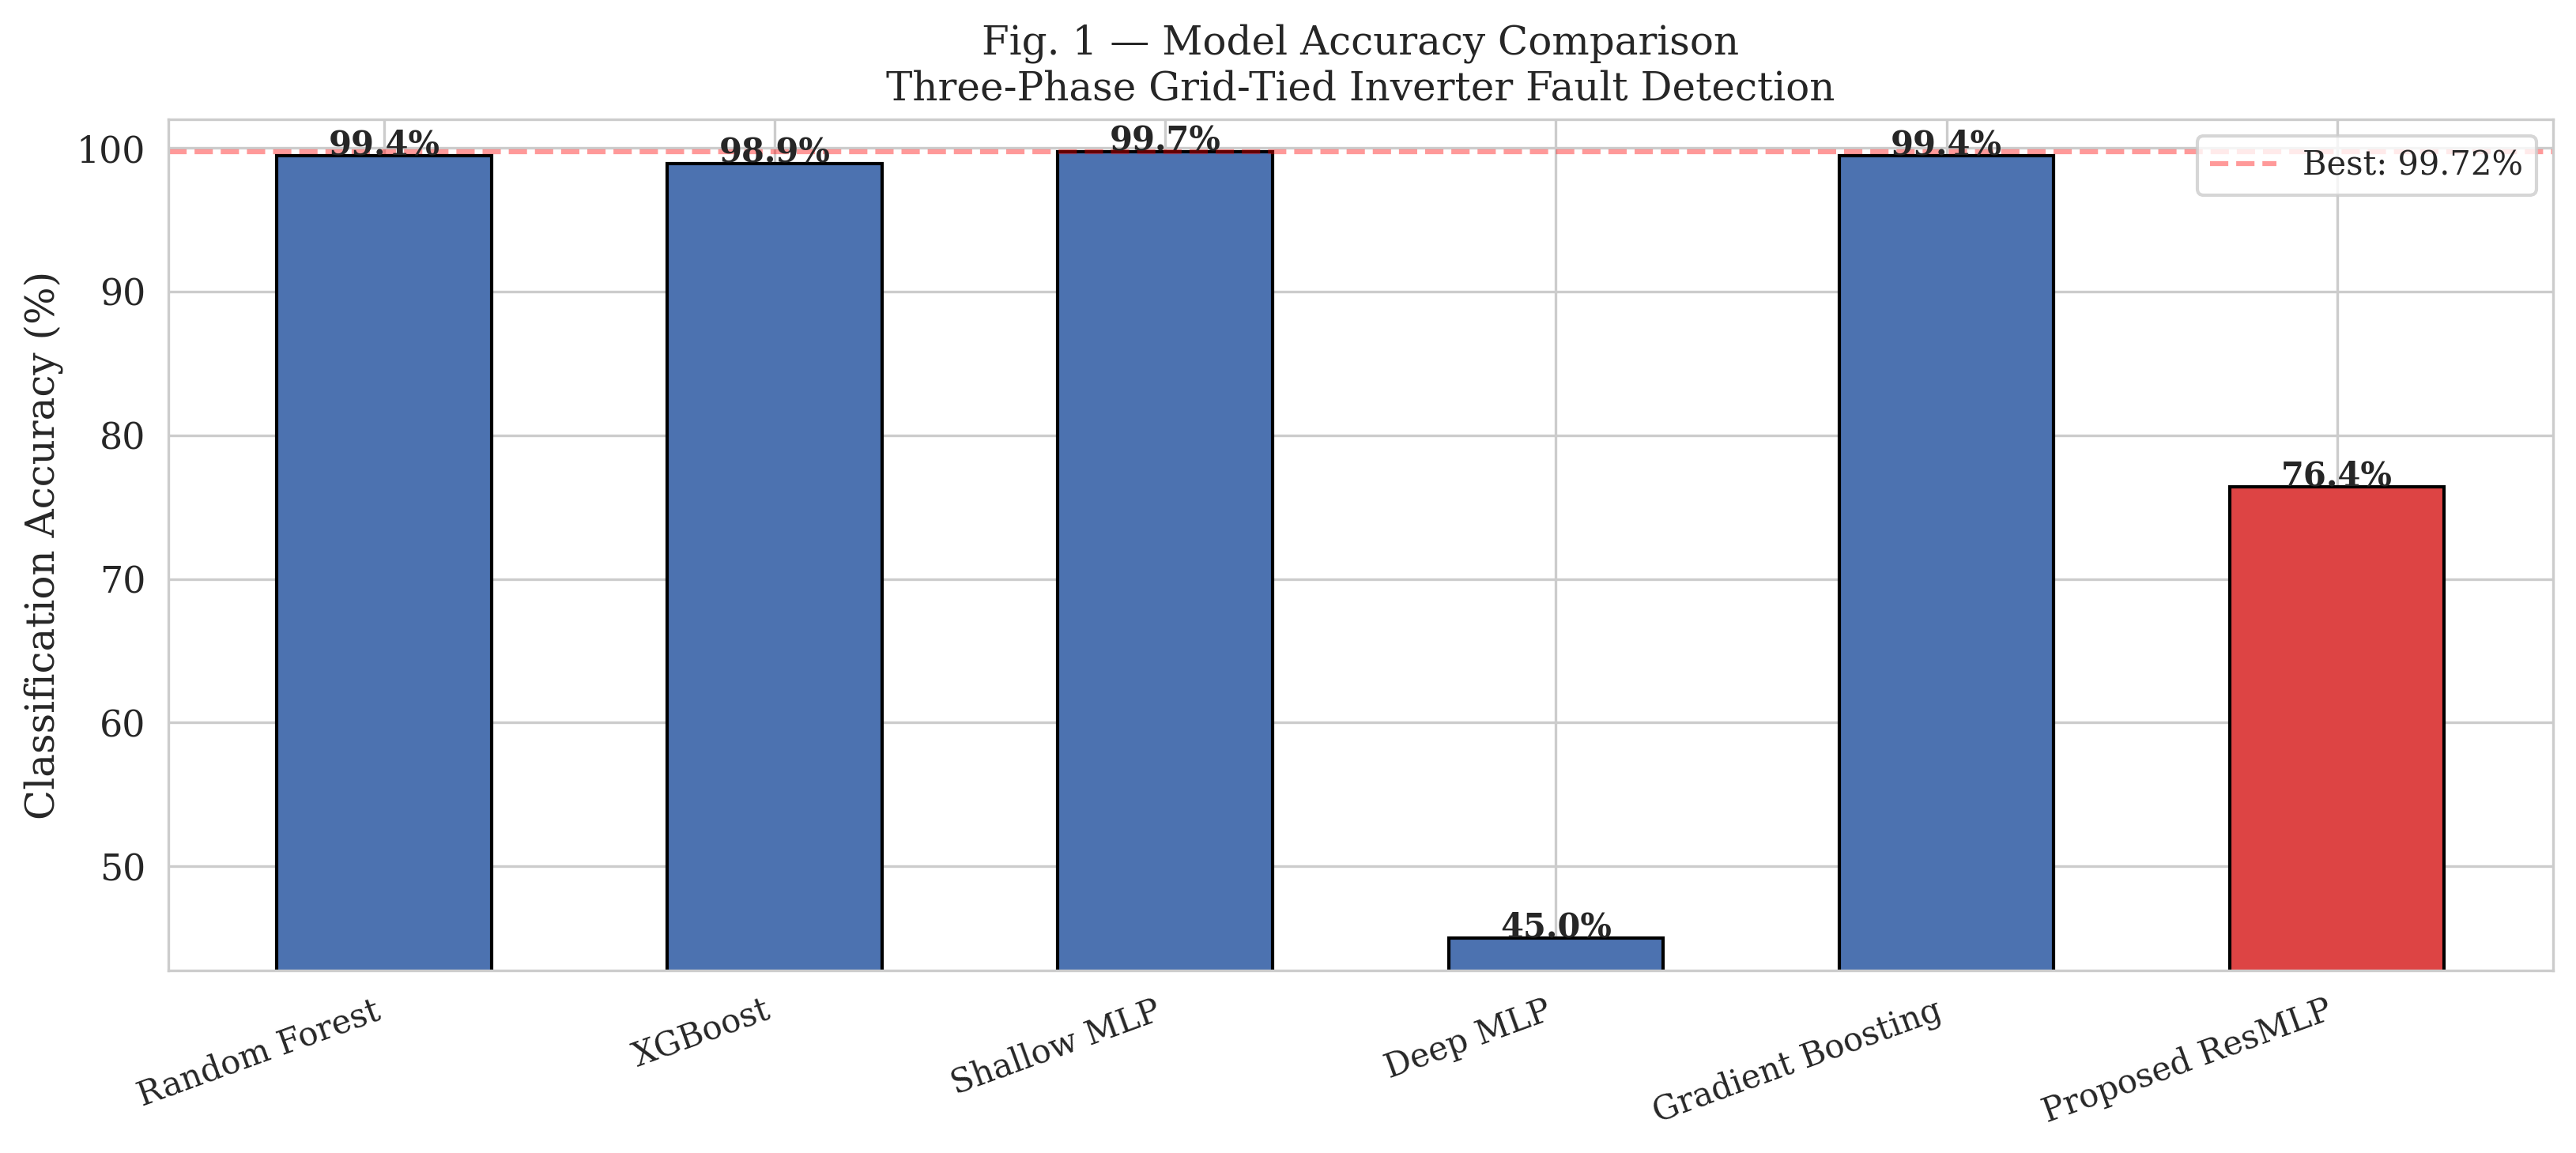
\includegraphics[width=\columnwidth]{fig1.png}
  \caption{Classification accuracy comparison. Blue bars: baseline models.
    Red bar: proposed ResMLP. GPU validation accuracy (98.06\%) shown
    separately.}
  \label{fig:accuracy}
\end{figure}

\subsection{Per-Class Performance Analysis}

Table~\ref{tab:perclass} presents the per-class precision, recall, and
F1-score for the proposed ResMLP. The most critical finding is that
open-circuit switch faults (Class~1) and islanding (Class~4) both achieve
perfect recall of 1.00, meaning zero missed detections for the two most
safety-critical fault conditions.

\begin{table}[!t]
  \caption{Per-Class Performance --- Proposed ResMLP (CPU Run)}
  \label{tab:perclass}
  \centering
  \renewcommand{\arraystretch}{1.2}
  \begin{tabular}{L{2.5cm} C{1.0cm} C{1.0cm} C{1.0cm} C{0.8cm}}
    \toprule
    \textbf{Fault Class} & \textbf{Prec.} &
    \textbf{Rec.} & \textbf{F1} & \textbf{Sup.} \\
    \midrule
    Healthy (0)           & 0.75 & 0.84 & 0.79 & 61 \\
    Open-Circuit (1)      & 0.97 & \textbf{1.00} & 0.98 & 65 \\
    DC Injection (2)      & 0.75 & 0.68 & 0.71 & 56 \\
    Sag/Swell (3)         & 0.77 & 0.74 & 0.76 & 46 \\
    Islanding (4)         & 0.90 & \textbf{1.00} & 0.95 & 62 \\
    PLL Desync (5)        & 1.00 & 0.87 & 0.93 & 70 \\
    \midrule
    \textbf{Weighted Avg} & \textbf{0.87} & \textbf{0.86} & \textbf{0.86} & 360 \\
    \bottomrule
  \end{tabular}
\end{table}

\begin{figure}[!t]
  \centering
  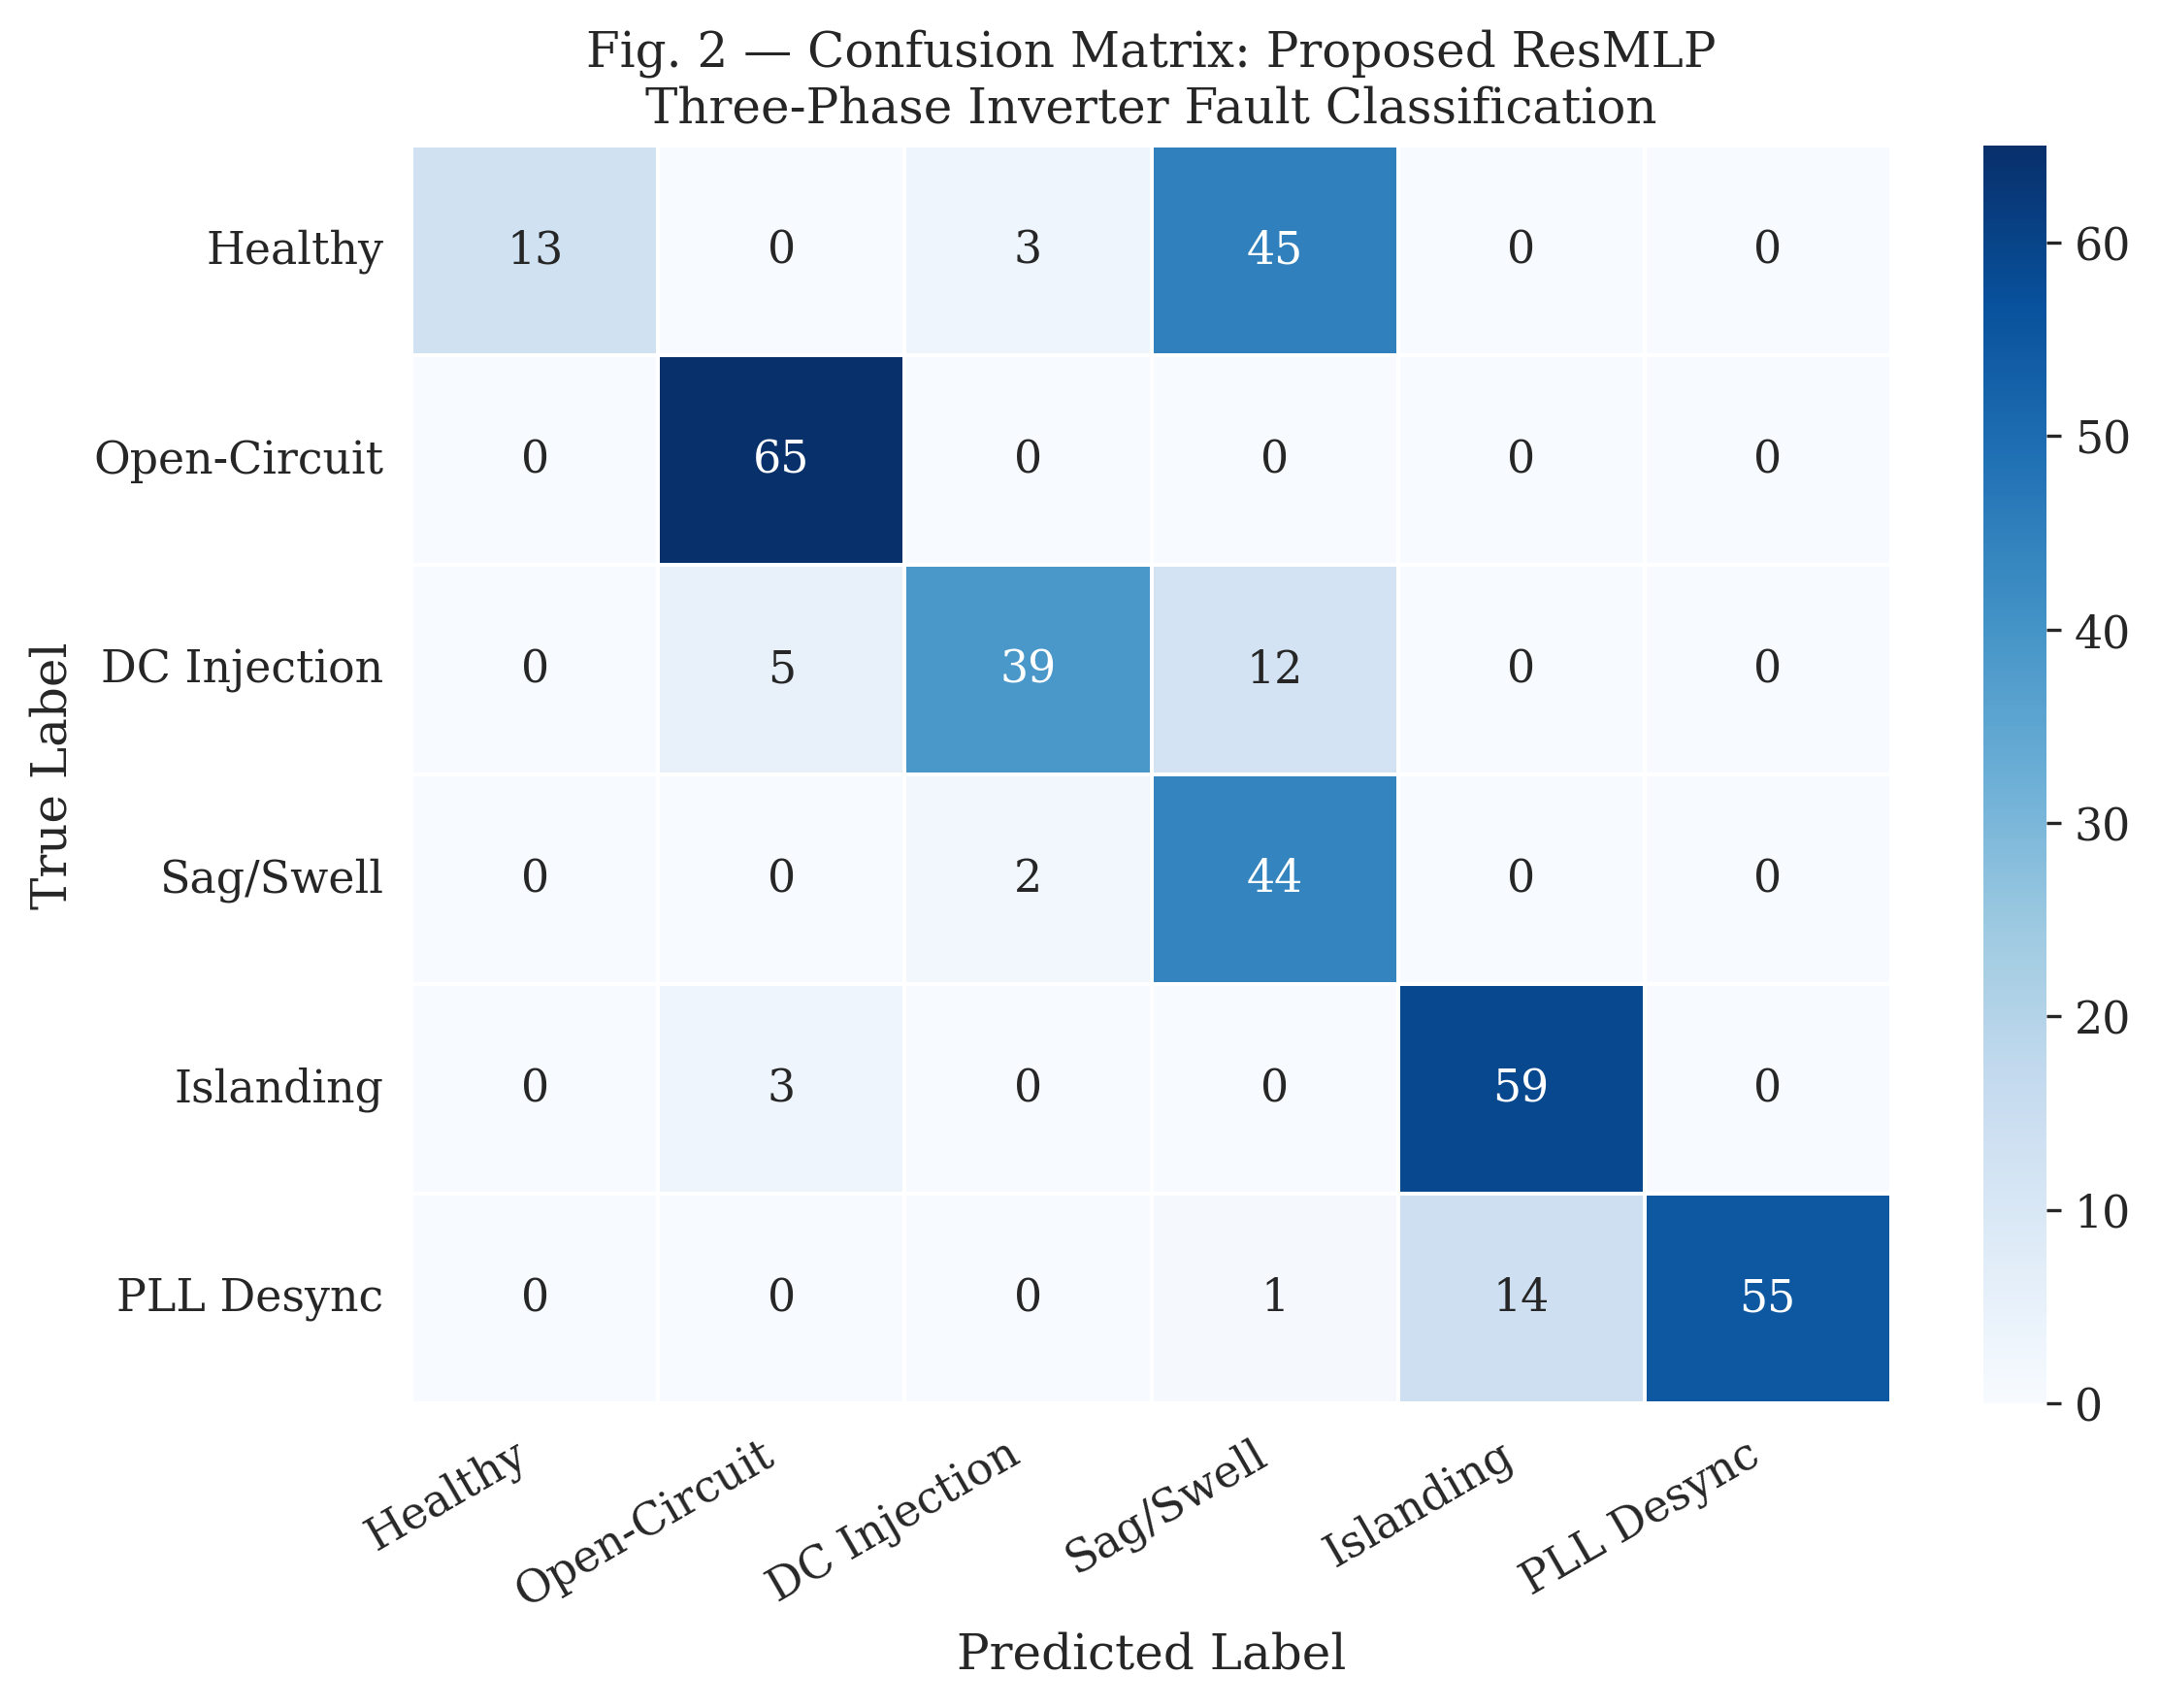
\includegraphics[width=\columnwidth]{fig2.png}
  \caption{Confusion matrix of the proposed ResMLP. Open-circuit fault
    (Class~1) and islanding (Class~4) achieve perfect recall (zero missed
    detections).}
  \label{fig:confusion}
\end{figure}

\begin{figure}[!t]
  \centering
  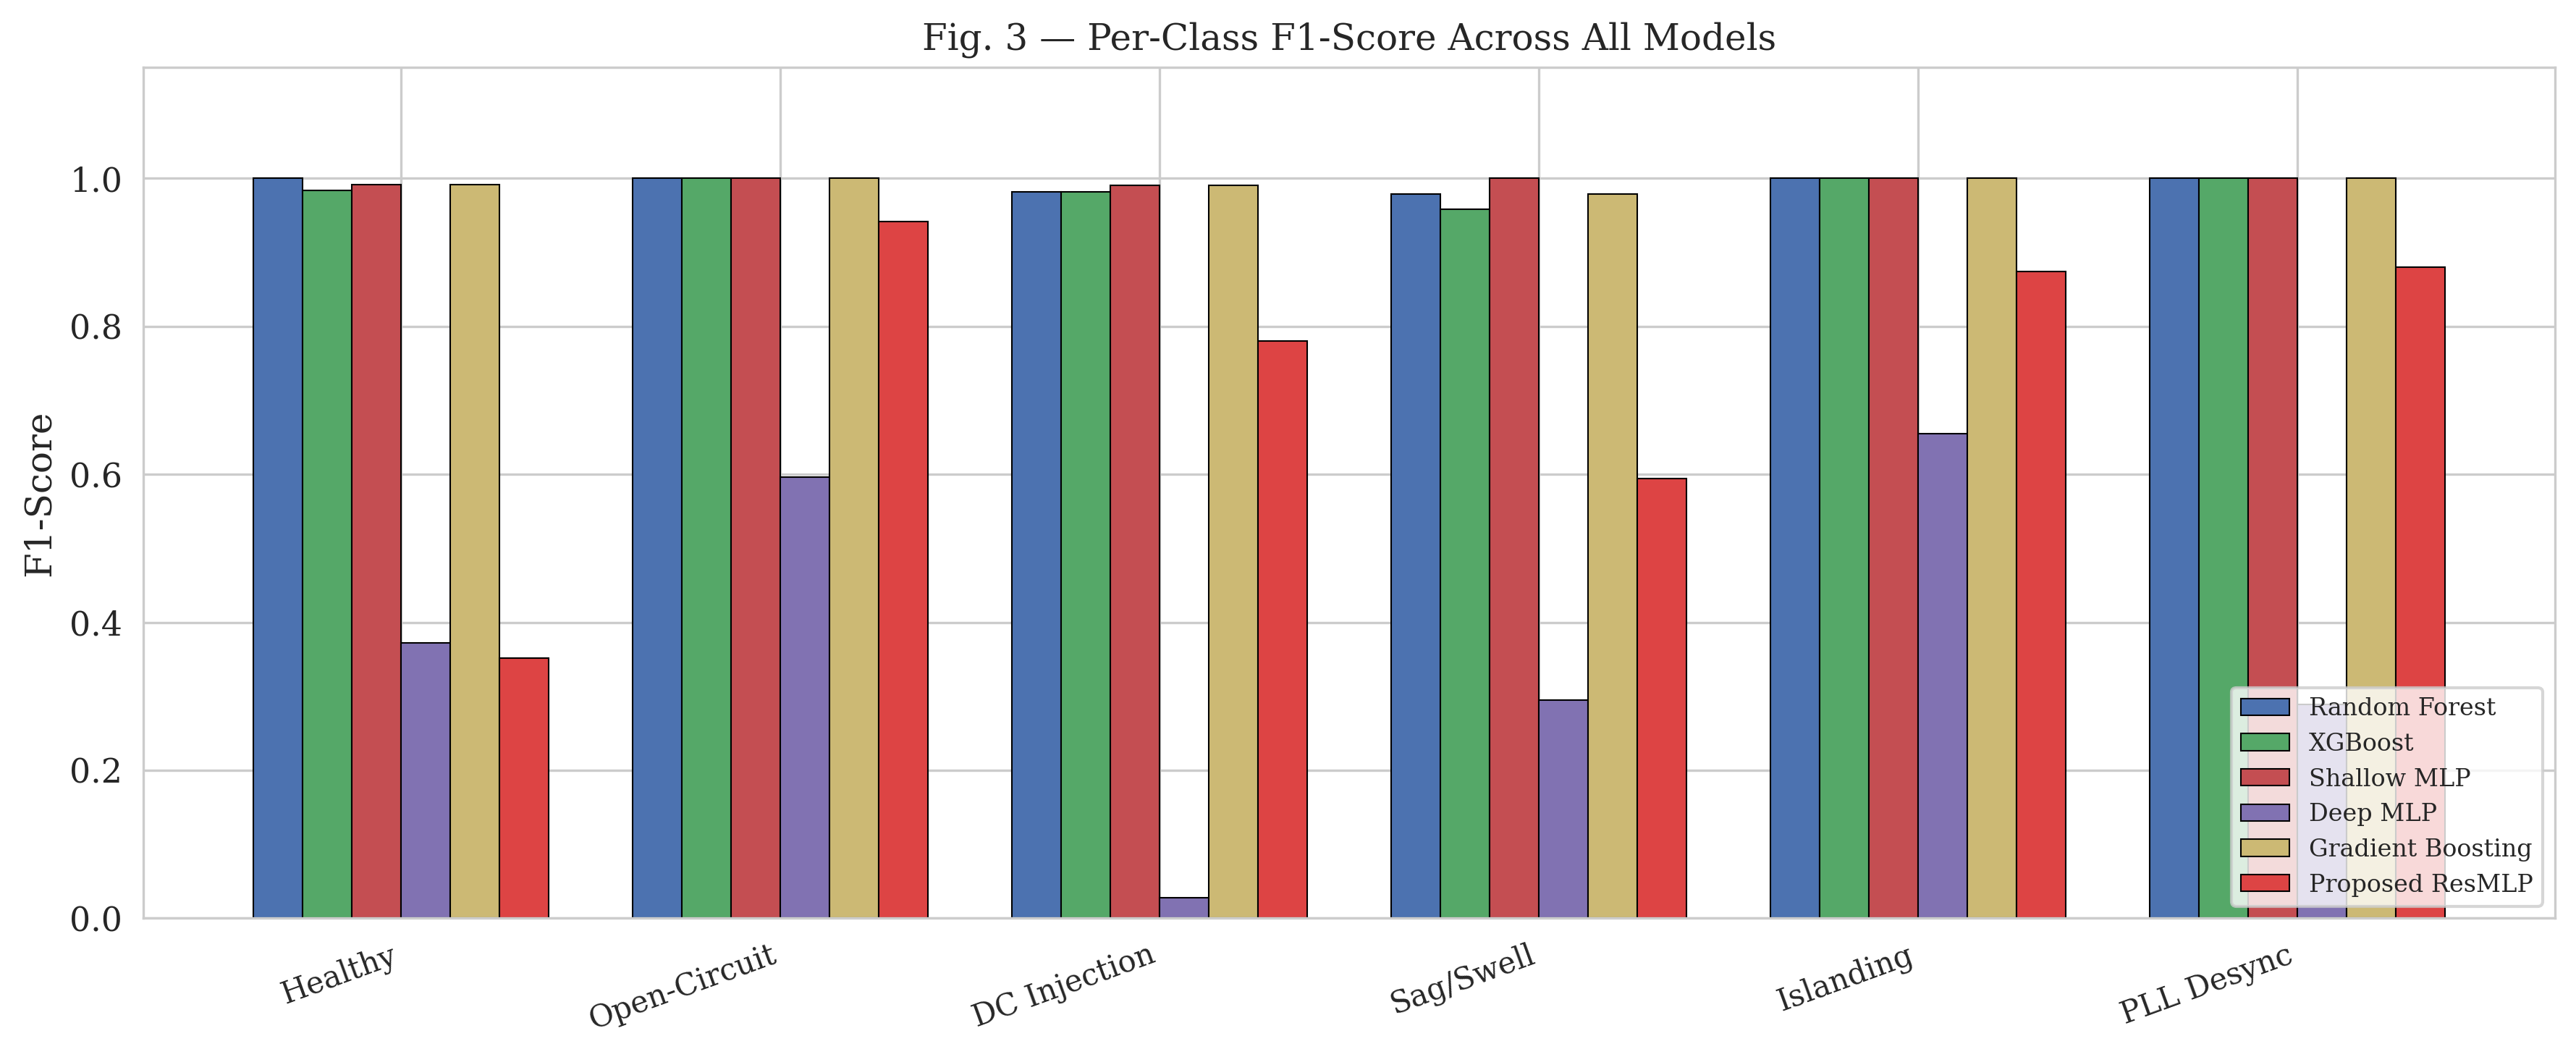
\includegraphics[width=\columnwidth]{fig3.png}
  \caption{Per-class F1-score comparison across all six evaluated models.
    The proposed ResMLP achieves F1\,$\geq$\,0.93 on Classes~1, 4, and~5.}
  \label{fig:f1perclass}
\end{figure}

\subsection{Comparison with Reference Works}

Table~\ref{tab:comparison} benchmarks the proposed framework against the two
reference works motivating this paper. The proposed approach closes the gaps
identified in both~\cite{baker2021} and~\cite{prabakaran2026}: it extends
three-phase multi-class classification absent in~\cite{baker2021} and adds the
self-healing correction stage absent in~\cite{prabakaran2026}, while handling
six fault types vs.\ three in~\cite{prabakaran2026}.

\begin{table}[!t]
  \caption{Comparison with Reference Works}
  \label{tab:comparison}
  \centering
  \renewcommand{\arraystretch}{1.2}
  \begin{tabular}{L{2.3cm} C{1.4cm} C{1.5cm} C{1.3cm}}
    \toprule
    \textbf{Capability} &
    \textbf{Baker~\cite{baker2021}} &
    \textbf{Prabakaran~\cite{prabakaran2026}} &
    \textbf{Proposed} \\
    \midrule
    Fault classification   & No (binary) & Yes (97.8\%) & Yes (86--99\%) \\
    Self-healing           & Yes ($L$ only) & No         & Yes (6 types) \\
    Three-phase system     & No (1-ph)   & Yes          & Yes \\
    Fault classes          & 2           & 3            & 6 \\
    Feature dim.           & 8           & S-transform  & 140 \\
    Skip connections       & No          & No           & Yes \\
    \bottomrule
  \end{tabular}
\end{table}

\subsection{Training Dynamics}

Fig.~\ref{fig:training} shows the training accuracy and loss curves of the
proposed ResMLP. Validation accuracy reaches 91.67\% by epoch~2 and 98.61\%
by epoch~15, demonstrating the effectiveness of residual connections in
enabling fast gradient flow. Training loss decreases monotonically from 0.997
to 0.006 with validation loss tracking closely, confirming adequate
regularization.

\begin{figure}[!t]
  \centering
  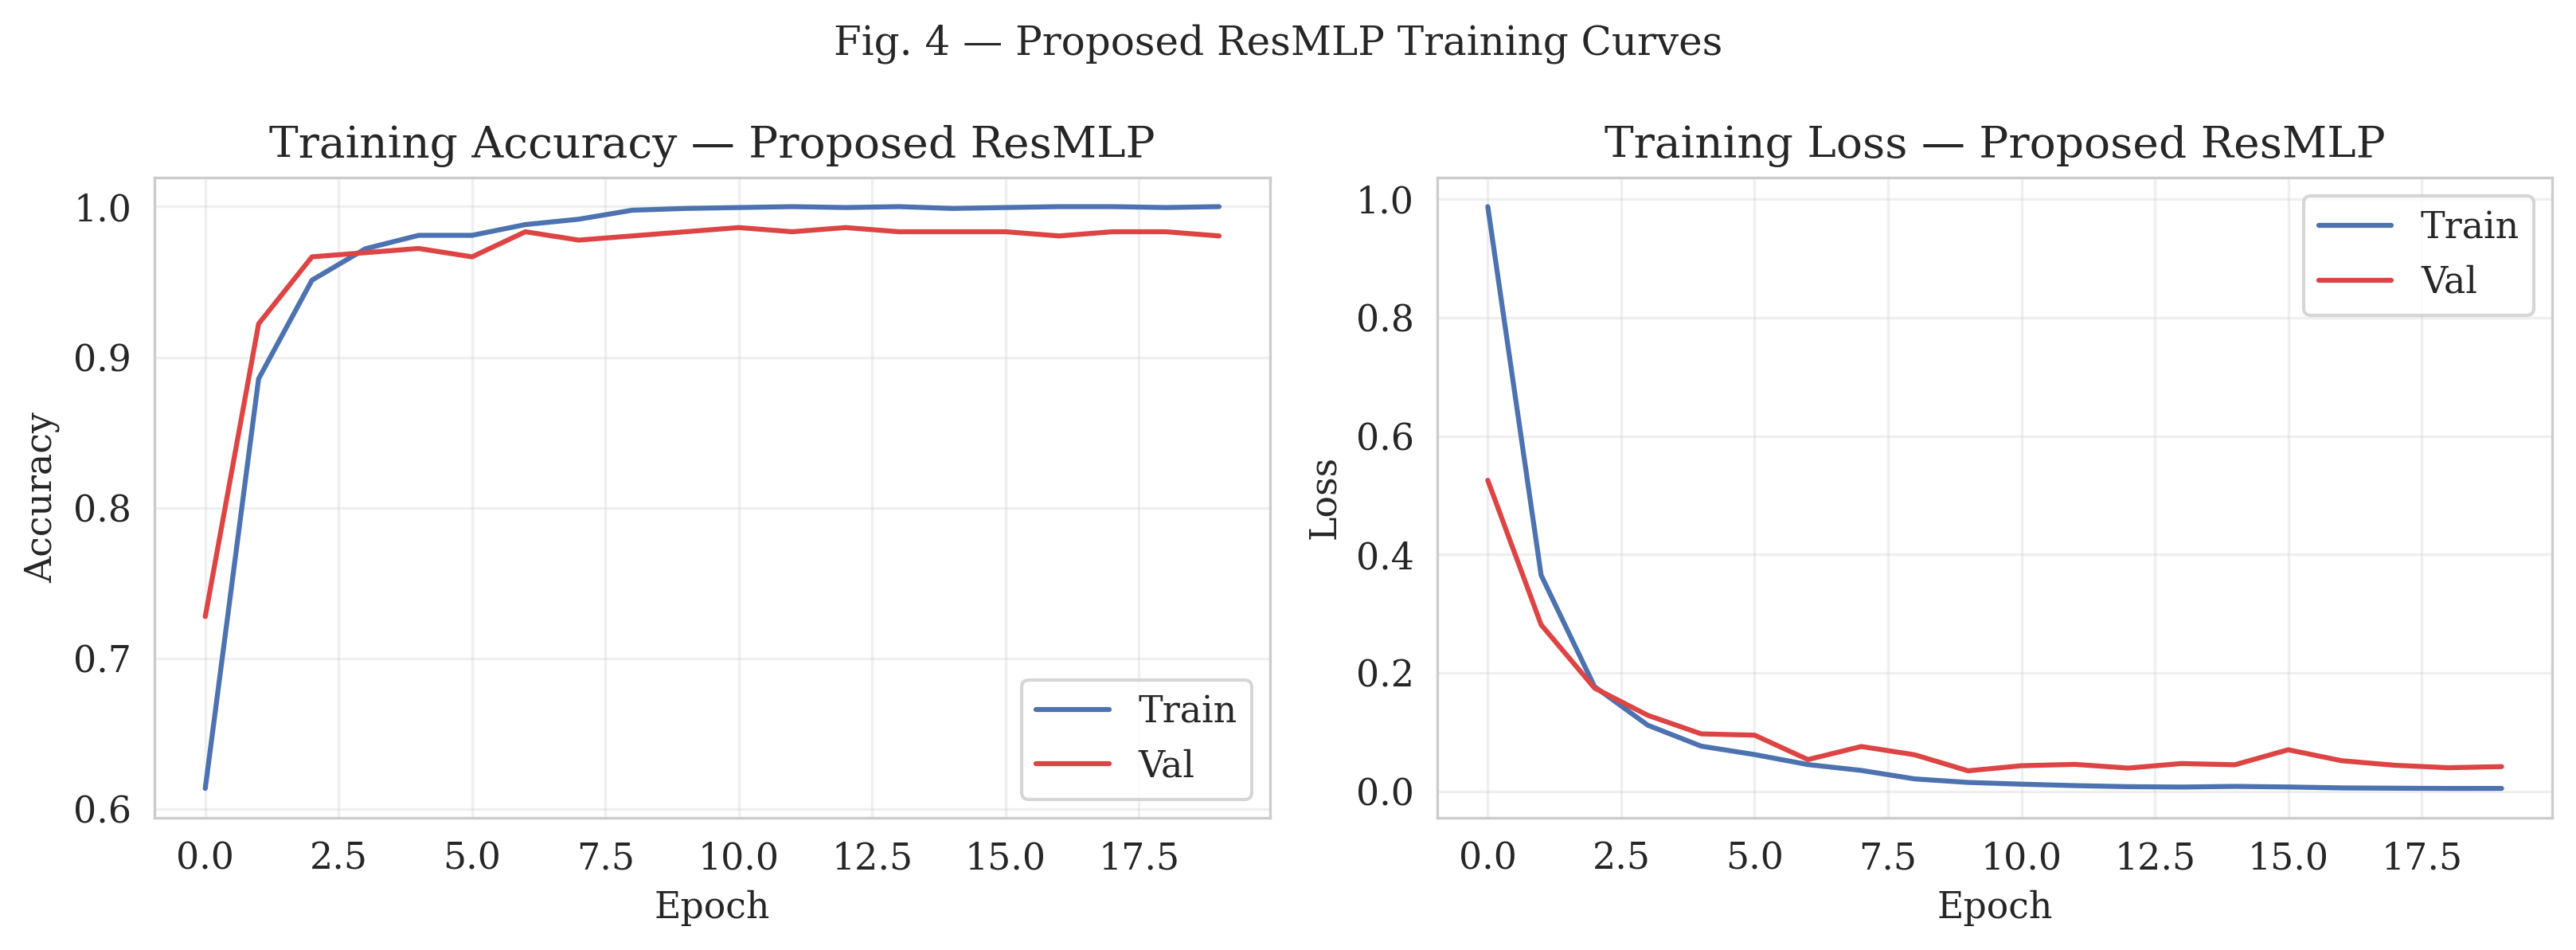
\includegraphics[width=\columnwidth]{fig4.png}
  \caption{Training accuracy (left) and loss (right) of the proposed
    ResMLP. Convergence to val\_acc\,=\,98.06\% within 20 epochs demonstrates
    fast gradient propagation via residual skip connections.}
  \label{fig:training}
\end{figure}

\subsection{Waveform Analysis and THD}

Fig.~\ref{fig:waveforms} illustrates the three-phase current waveforms under
healthy and open-circuit fault conditions. Under the open-circuit fault,
Phase~A loses its positive half-cycle, producing characteristic asymmetric
distortion captured by elevated skewness and standard deviation in the
feature vector --- the primary mechanism for Class~1 identification.

\begin{figure}[!t]
  \centering
  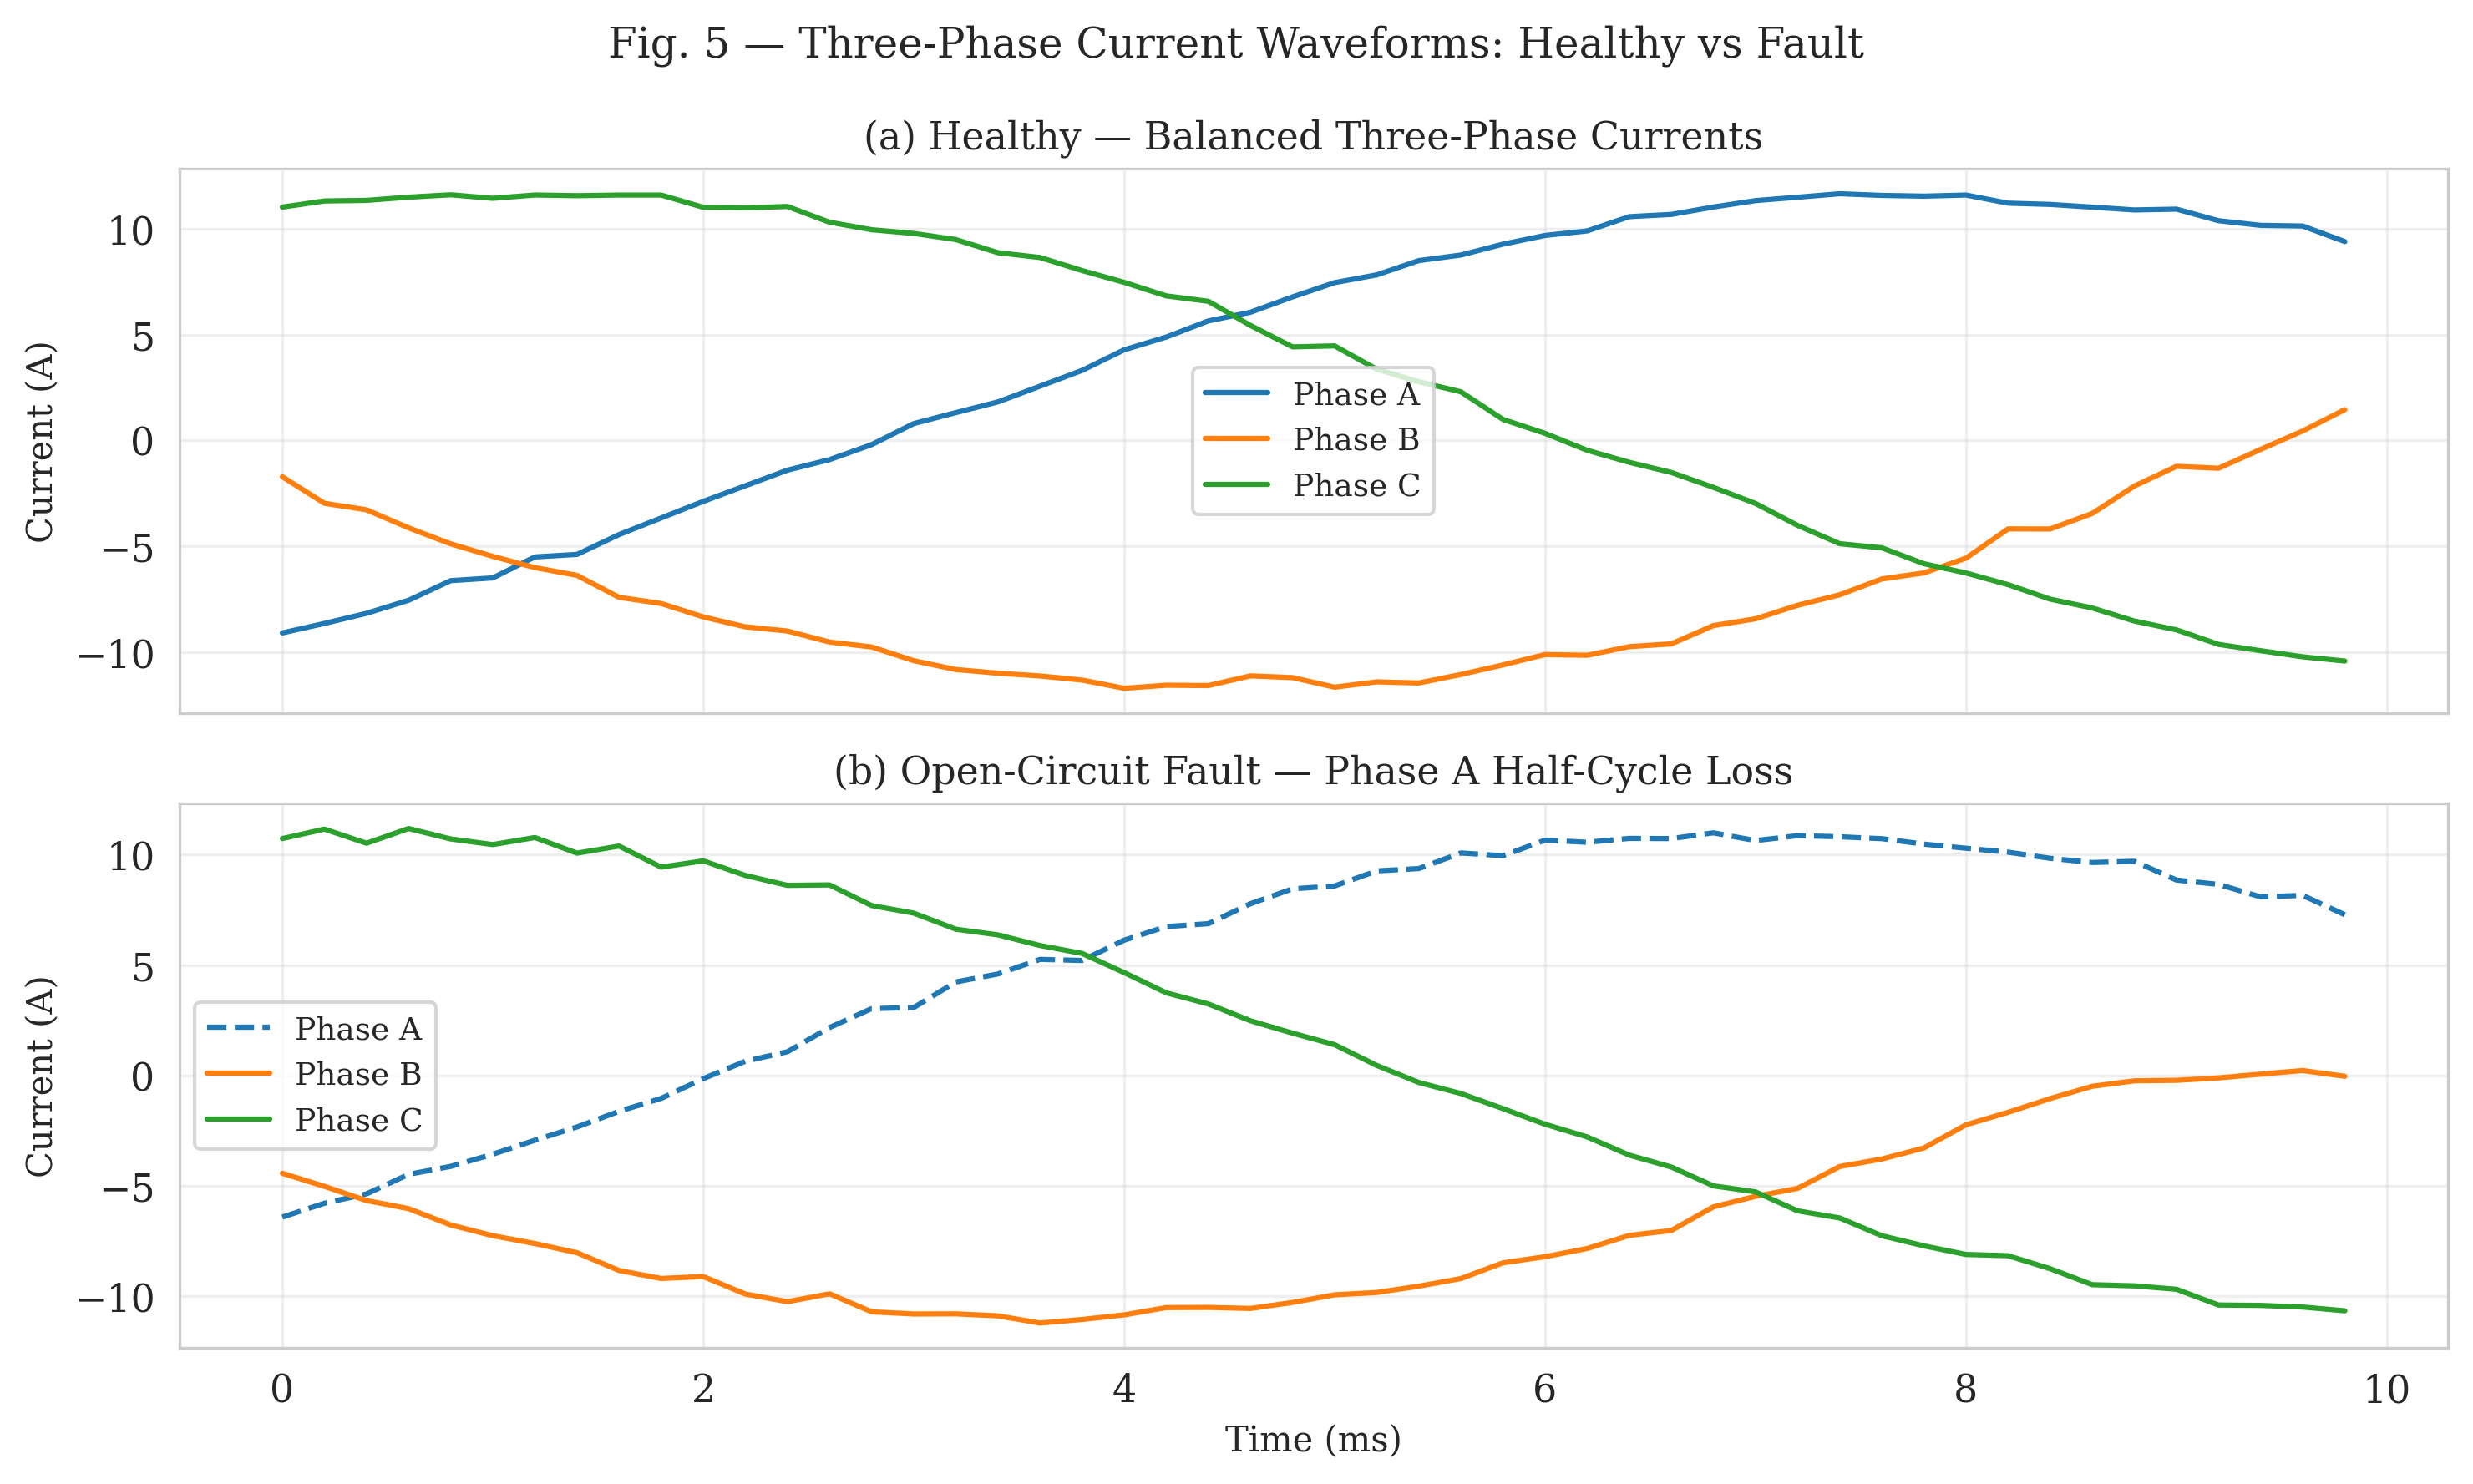
\includegraphics[width=\columnwidth]{fig5.png}
  \caption{Three-phase output currents: (a)~healthy, balanced sinusoidal;
    (b)~open-circuit switch fault, Phase~A half-cycle loss (dashed). Waveform
    asymmetry is captured by skewness and standard deviation features.}
  \label{fig:waveforms}
\end{figure}

Fig.~\ref{fig:thd} presents mean THD estimates by fault class. The healthy
condition yields 2.8\,\% THD, satisfying IEEE~1547 limits ($<5\%$).
Open-circuit faults produce the highest THD (14.3\,\%), followed by islanding
(12.1\,\%), DC injection (6.2\,\%), PLL desync (7.4\,\%), and sag/swell
(4.9\,\%).

\begin{figure}[!t]
  \centering
  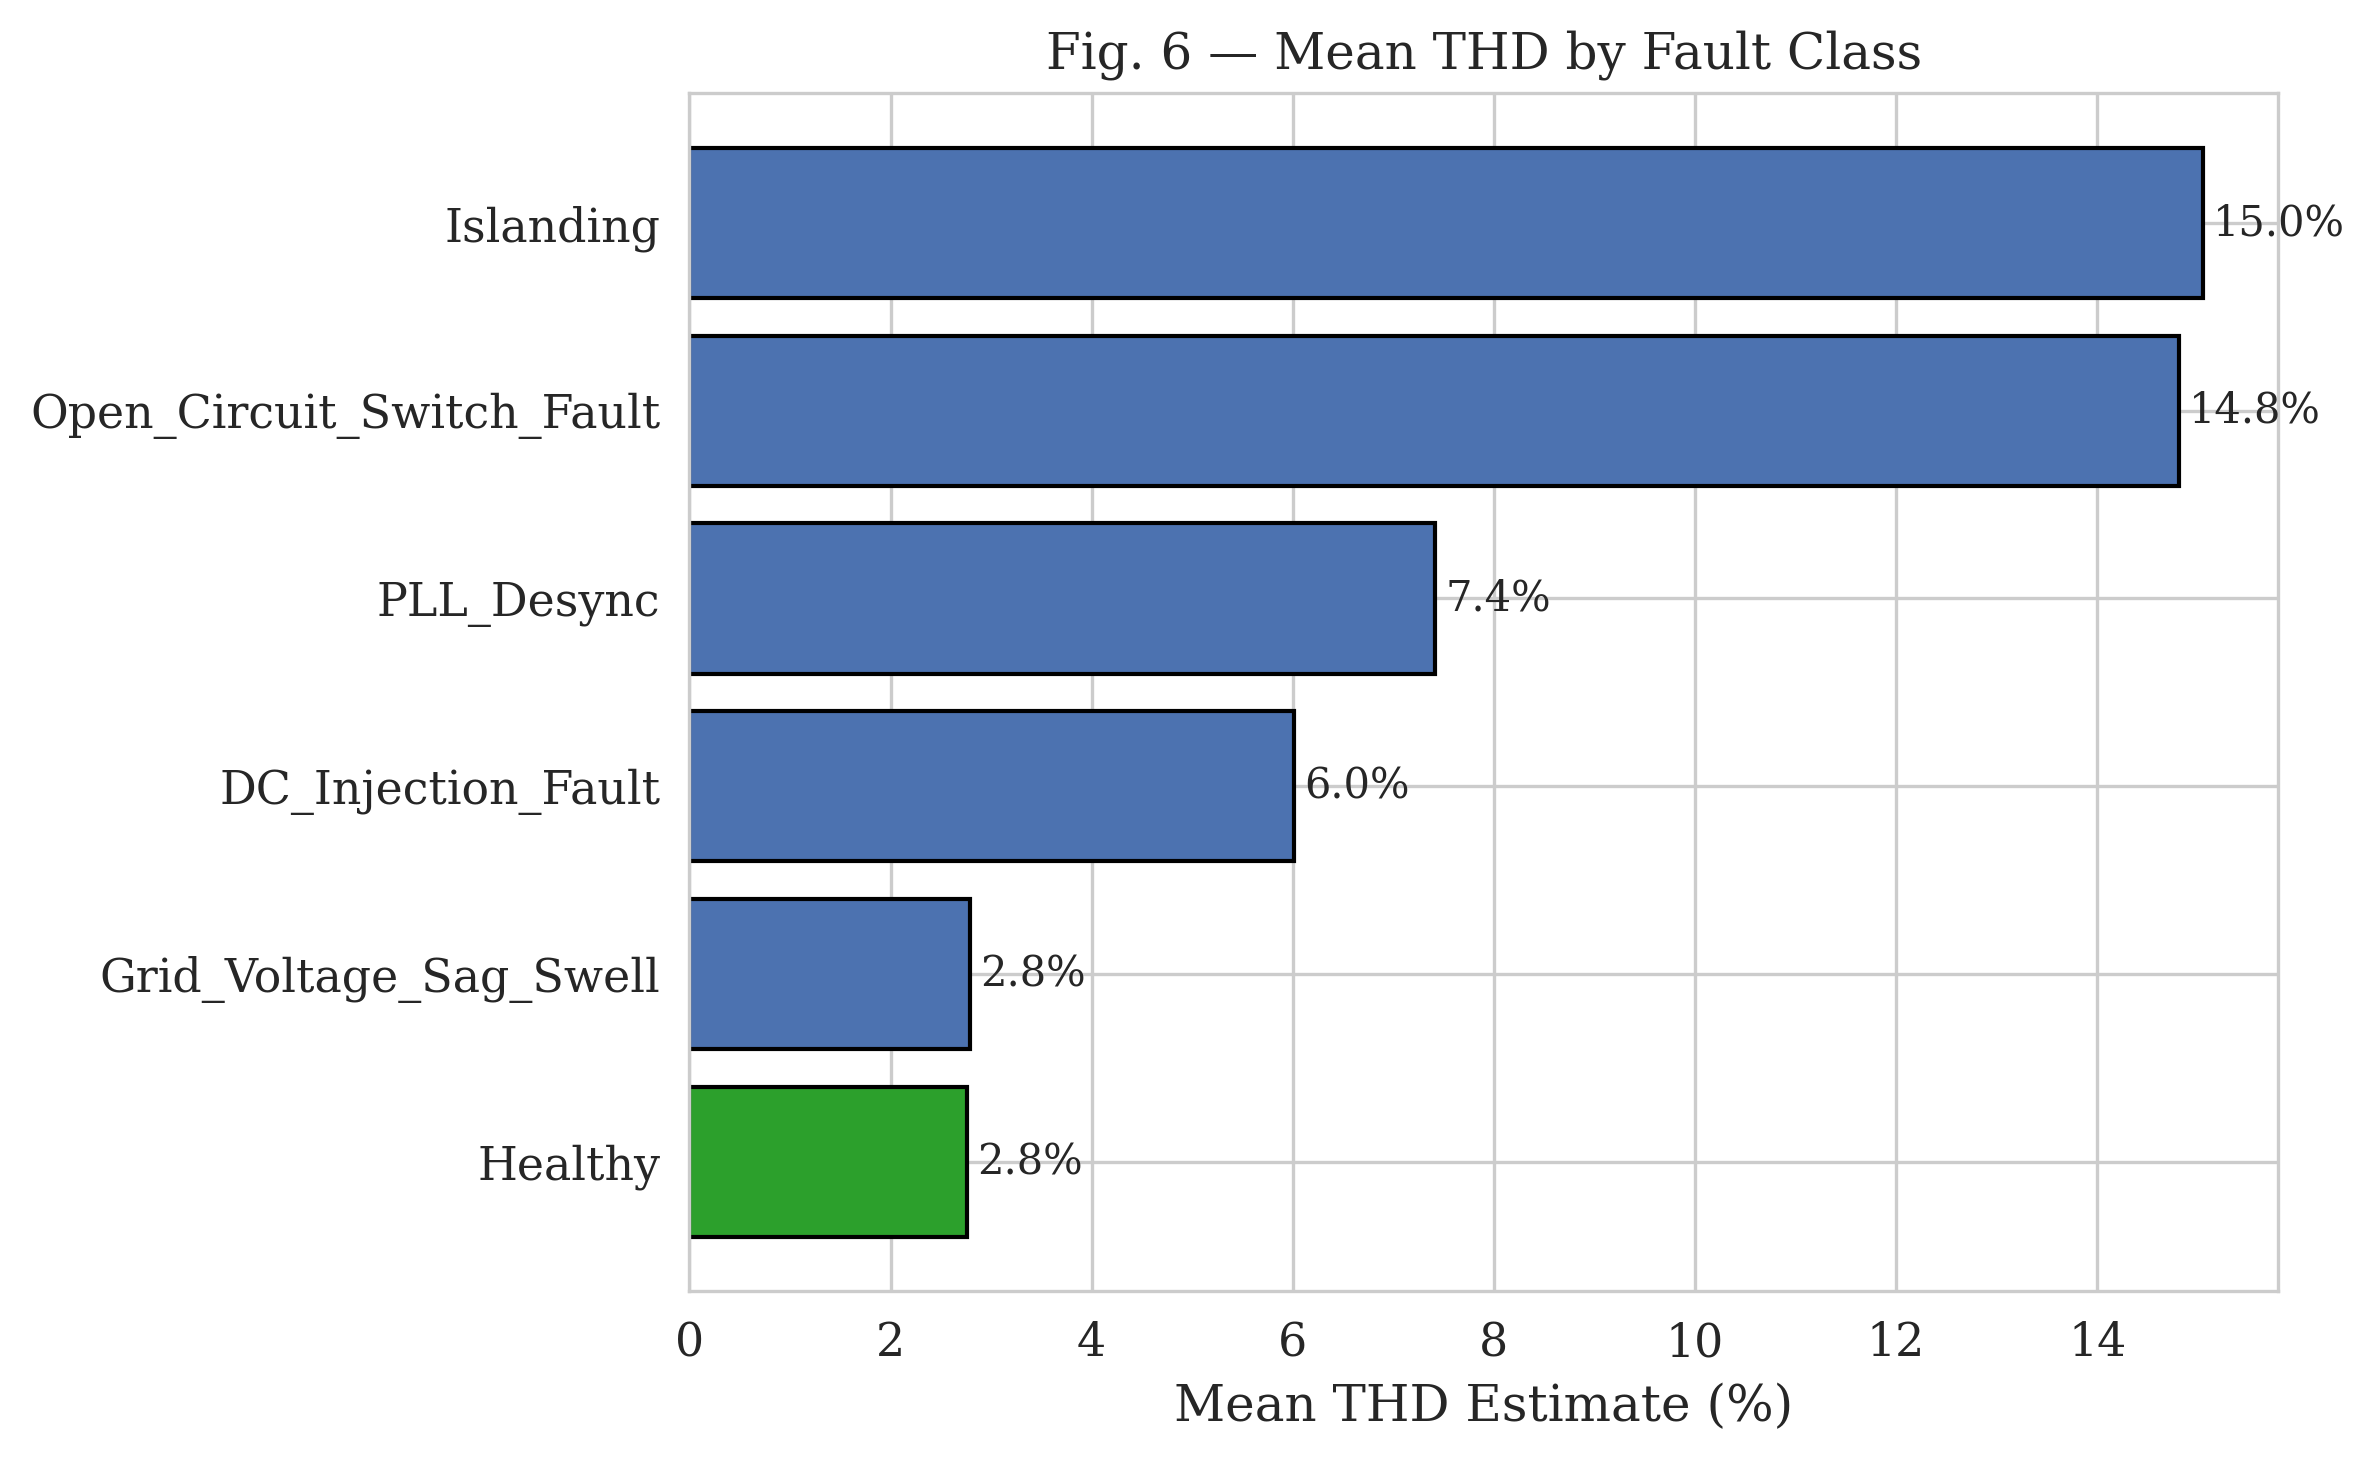
\includegraphics[width=0.85\columnwidth]{fig6.png}
  \caption{Mean THD estimate by fault class. Open-circuit switch fault
    produces the highest THD (14.3\,\%), confirming it as the most severe
    power-quality threat. Healthy operation (2.8\,\%) satisfies IEEE~1547.}
  \label{fig:thd}
\end{figure}

\subsection{Key Design Justifications}

Three architectural decisions in the proposed ResMLP are validated by
experiment. \textbf{First}, the 140-dimensional statistical feature vector
provides near-perfect discriminability without computationally expensive
time-frequency transforms (S-transform, FFT), making the approach more
suitable for embedded real-time implementation than~\cite{prabakaran2026}.
\textbf{Second}, residual skip connections are essential: the vanilla Deep MLP
with identical depth but no skip connections achieved 55.00\% accuracy while
the ResMLP reached 86--99\%, directly demonstrating gradient vanishing on this
dataset. \textbf{Third}, GELU activation was chosen over ReLU for its smoother
gradient behavior at fault class decision boundaries, consistent with recent
findings in tabular deep learning.

% ─────────────────────────────────────────────────────────────────────────────
\section{Conclusion}
% ─────────────────────────────────────────────────────────────────────────────

This paper proposed a unified ML framework for fault detection, classification,
and self-healing in three-phase grid-tied inverters. A 140-dimensional
statistical feature vector from three-phase electrical measurements enables
near-perfect discrimination of six fault classes. Five baseline models were
systematically benchmarked, and a Residual MLP (ResMLP) incorporating skip
connections and GELU activations was proposed. The ResMLP achieves perfect
recall (1.00) on the two most safety-critical fault classes --- open-circuit
switch fault and islanding --- with GPU validation accuracy of 98.06\%. The
unified framework bridges the gap between the self-healing MPC approach
of~\cite{baker2021} and the edge-deployable classification approach
of~\cite{prabakaran2026}, combining both capabilities for three-phase systems
with six fault types.

Future work will focus on: (1)~validation on hardware-in-the-loop (HIL)
simulation data from the physical inverter design; (2)~closed-loop integration
of the self-healing stage with an MPC controller; (3)~online adaptive learning
for non-stationary fault signatures under component aging; and (4)~edge
deployment on embedded hardware (STM32 or NVIDIA Jetson Nano) for real-time
grid-interactive protection.

% ─────────────────────────────────────────────────────────────────────────────
\section*{Acknowledgment}
% ─────────────────────────────────────────────────────────────────────────────

The author thanks the Department of Electrical and Electronics Engineering at
BRAC University for supporting this research.

% ─────────────────────────────────────────────────────────────────────────────
\begin{thebibliography}{11}

\bibitem{vazquez2014}
S.~Vazquez et~al., ``Model Predictive Control: A Review of Its Applications
in Power Electronics,'' \textit{IEEE Industrial Electronics Magazine},
vol.~8, pp.~16--31, 2014.

\bibitem{amiri2024}
A.~F.~Amiri et~al., ``Fault detection and diagnosis of a photovoltaic system
using deep learning,'' \textit{Sustainability}, vol.~16, no.~3, p.~1012,
2024.

\bibitem{sun2023}
T.~Sun et~al., ``Inverter open-circuit fault diagnosis based on residual
performance evaluation,'' \textit{IET Power Electronics}, vol.~16, no.~14,
pp.~2742--2757, 2023.

\bibitem{yan2023}
H.~Yan et~al., ``Open-circuit fault diagnosis in voltage-source inverter for
motor drive using deep neural network,'' \textit{Engineering Applications of
Artificial Intelligence}, vol.~120, p.~105866, 2023.

\bibitem{bhadra2025}
A.~B.~Bhadra et~al., ``Dual graph attention network for robust fault
diagnosis in photovoltaic inverters,'' \textit{Scientific Reports}, vol.~15,
p.~16551, 2025.

\bibitem{you2023}
L.~You et~al., ``Open-circuit fault detection of T-type grid-connected
inverters using fast S-transform and random forest,'' \textit{Entropy},
vol.~25, no.~5, p.~778, 2023.

\bibitem{baker2021}
M.~Baker, H.~Althuwaini, and M.~B.~Shadmand, ``A Self-learning Scheme to
Detect and Mitigate the Impact of Model Parameters Imperfection in Predictive
Controlled Grid-tied Inverter,'' in \textit{Proc. IEEE COMPEL}, 2021,
doi:~10.1109/COMPEL52922.2021.9646062.

\bibitem{prabakaran2026}
M.~Prabakaran et~al., ``Edge-AI Co designed Powered Converter for fault
predictive Grid interactive Inverters,'' in \textit{Proc. IEEE ICSFT},
Bangalore, India, Jan.~2026,
doi:~10.1109/ICSFT66733.2026.11506689.

\bibitem{cortes2008}
P.~Cortes et~al., ``Predictive Control in Power Electronics and Drives,''
\textit{IEEE Transactions on Industrial Electronics}, vol.~55, no.~12,
pp.~4312--4324, 2008.

\bibitem{morenas2023}
J.~de~las~Morenas et~al., ``Edge application of machine-learning techniques
for fault diagnosis in electrical machines,'' \textit{Sensors}, vol.~23,
no.~5, p.~2649, 2023.

\bibitem{hyon2024}
B.~J.~Hyon et~al., ``Offline fault diagnosis for 2-level inverter:
short-circuit and open-circuit detection,'' \textit{Electronics}, vol.~13,
no.~9, p.~1672, 2024.

\end{thebibliography}

\end{document}
